\documentclass[12pt]{article}

\usepackage[final]{graphicx}
\usepackage[final]{fixme}
\fxsetup{layout=footnote}
\usepackage[left]{lineno}
\usepackage{tikz-feynman}
\usepackage{amsmath,amsthm,amssymb,mathtools,caption,subcaption,mathrsfs,cancel,multirow,enumitem,setspace,sectsty,cite,hyperref,siunitx,cancel}
\usepackage{fullpage}

\sectionfont{\large}
\subsectionfont{\normalsize}

\newcommand{\SUthreecSUtwoLUoneY}{\mathrm{SU} {\left(3\right)}_c {\times} \mathrm{SU} {\left(2\right)}_L {\times} \mathrm{U} {\left(1\right)}_Y}
\newcommand{\SUtwoUone}{\mathrm{SU} {\left(2\right)} {\times} \mathrm{U} {\left(1\right)}}
\newcommand{\SUtwoLUoneY}{\mathrm{SU} {{\left(2\right)}}_L {\times} \mathrm{U} {\left(1\right)}_Y}
\newcommand{\SUthreec}{\mathrm{SU} {\left(3\right)}_c}
\newcommand{\SUtwoL}{\mathrm{SU} {\left(2\right)}_L}
\newcommand{\SUtwo}{\mathrm{SU} {\left(2\right)}}
\newcommand{\UoneY}{\mathrm{U} {\left(1\right)}_Y}
\newcommand{\UoneQ}{\mathrm{U} {\left(1\right)}_Q}
\newcommand{\Uone}{\mathrm{U} {\left(1\right)}}
\newcommand{\custodialSymmetry}{\mathrm{SU} {\left(2\right)}_L {\times} \mathrm{SU} {\left(2\right)}_R}
\newcommand{\CP}{\mathrm{CP}}

\newcommand{\lepL}{\mathrm{L}_\ell}
\newcommand{\quaL}{\mathrm{L}_{\mathrm{q}}}
\newcommand{\ellL}{\ell_L}
\newcommand{\uL}{\mathrm{u}_L}
\newcommand{\nuL}{\nu_L}
\newcommand{\dL}{\mathrm{d}_L}
\newcommand{\lepR}{\mathrm{R}_\ell}
\newcommand{\uQuaR}{\mathrm{R}_{\mathrm{u}}}
\newcommand{\dQuaR}{\mathrm{R}_{\mathrm{d}}}
\newcommand{\ellR}{\ell_R}
\newcommand{\uR}{\mathrm{u}_R}
\newcommand{\dR}{\mathrm{d}_R}

\newcommand{\lepLBar}{\bar{\mathrm{L}}_\ell}
\newcommand{\quaLBar}{\bar{\mathrm{L}}_{\mathrm{q}}}
\newcommand{\ellLBar}{\bar{\ell}_L}
\newcommand{\uLBar}{\bar{u}_L}
\newcommand{\nuLBar}{\bar{\nu}_L}
\newcommand{\dLBar}{\bar{d}_L}
\newcommand{\lepRBar}{\bar{\mathrm{R}}_\ell}
\newcommand{\uQuaRBar}{\bar{\mathrm{R}}_u}
\newcommand{\dQuaRBar}{\bar{\mathrm{R}}_d}
\newcommand{\ellRBar}{\bar{\ell}_R}
\newcommand{\uRBar}{\bar{u}_R}
\newcommand{\dRBar}{\bar{d}_R}
\newcommand{\ttbar}{\mathrm{t}\bar{\mathrm{t}}}

\newcommand{\Z}{\mathrm{Z}}
\newcommand{\Wp}{\mathrm{W}^+}
\newcommand{\Wm}{\mathrm{W}^-}
\newcommand{\Wpm}{\mathrm{W}^\pm}
\newcommand{\W}{\mathrm{W}}
\newcommand{\V}{\mathrm{V}}
\newcommand{\Higgs}{\mathrm{H}}
\newcommand{\higgs}{\mathrm{h}}
\newcommand{\A}{\mathrm{A}}
\newcommand{\g}{\mathrm{g}}
\newcommand{\f}{\mathrm{f}}
\newcommand{\sfermion}{\tilde{\mathrm{f}}}
\newcommand{\fBar}{\bar{\mathrm{f}}}
\newcommand{\q}{\mathrm{q}}
\newcommand{\qBar}{\bar{\mathrm{q}}}
\newcommand{\e}{\mathrm{e}}
\newcommand{\p}{\mathrm{p}}
\newcommand{\tQ}{\mathrm{t}}
\newcommand{\tQBar}{\bar{\mathrm{t}}}
\newcommand{\bQ}{\mathrm{b}}
\newcommand{\bQBar}{\bar{\mathrm{b}}}
\newcommand{\cQ}{\mathrm{c}}
\newcommand{\cQBar}{\bar{\mathrm{c}}}
\newcommand{\sQ}{\mathrm{s}}
\newcommand{\sQBar}{\bar{\mathrm{s}}}
\newcommand{\uQ}{\mathrm{u}}
\newcommand{\uQBar}{\bar{\mathrm{u}}}
\newcommand{\dQ}{\mathrm{d}}
\newcommand{\dQBar}{\bar{\mathrm{d}}}
\newcommand{\eL}{\mathrm{e}}

\newcommand{\ferLag}{\mathcal{L}_{\mathrm{fermion}}}
\newcommand{\gauLag}{\mathcal{L}_{\mathrm{gauge}}}
\newcommand{\scaLag}{\mathcal{L}_{\mathrm{scalar}}}

\newcommand{\MeV}{\,\mathrm{MeV}{}}
\newcommand{\GeV}{\,\mathrm{GeV}{}}
\newcommand{\TeV}{\,\mathrm{TeV}{}}
\newcommand{\fbinv}{\,\mathrm{fb}^{-1}{}}
\newcommand{\um}{\,\mathrm{\mu m}{}}
\newcommand{\m}{\,\mathrm{m}{}}
\newcommand{\cm}{\,\mathrm{cm}{}}
\newcommand{\T}{\,\mathrm{T}{}}
\newcommand{\kt}{\,\mathrm{kt}{}}
\newcommand{\GJ}{\,\mathrm{GJ}{}}
\newcommand{\stat}{\,\mathrm{(stat.)}{}}
\newcommand{\sys}{\,\mathrm{(sys.)}{}}
\newcommand{\s}{\,\mathrm{s}{}}
\newcommand{\MHz}{\,\mathrm{MHz}{}}
\newcommand{\km}{\,\mathrm{km}{}}
\newcommand{\kilo}{\,\mathrm{k}{}}

\newcommand{\absEta}{\left|\eta\right|}
\newcommand{\pt}{p_{\mathrm{T}}}
\newcommand{\thetaCS}{\theta_{\mathrm{CS}}}
\newcommand{\bsmBR}{\mathrm{BR}_{\mathrm{BSM}}}
\newcommand{\mPlanck}{M_{\mathrm{Pl}}}
\newcommand{\mHiggs}{M_{\mathrm{H}}}
\newcommand{\MET}{\cancel{\it{E}}_{T}}
\newcommand{\pT}{p_T}


\title{Naturalness and Long-Lived Beyond the Standard Model Particles}
\author{Bryan Cardwell}

\begin{document}

\pagenumbering{gobble}
\singlespacing
\maketitle

\begin{abstract}

I'll write an abstract here.

\end{abstract}

\newpage
\tableofcontents
\newpage
\doublespacing
\linenumbers
\pagenumbering{arabic}

% Things to check
\fxnote{When should symbols be italicized and when should they be mathrm'd?} 
\fxnote{fine-tuning or fine tuning?} 

\section{The Standard Model} \label{SM}
    The standard model of particle physics (SM) describes all known particles and their non-gravitational interactions and is experimentally verified to astonishing \fxnote{weak word} accuracy. The SM consists of \num{12} spin-$\frac{1}{2}$ particles, the fermions, that make up all observed matter; \num{12} spin-1 particles, the gauge bosons, that communicate the electromagnetic, weak, and strong forces; and one fundamental scalar, the Higgs boson, which will be described in detail below.
    
    All SM particles transform according to the gauged symmetry group\fxnote{be good at describing the meaning of `gauged symmetry group'} $\SUthreecSUtwoLUoneY$, where $\SUthreec$ is associated with color charge, $\SUtwoL$ is associated with weak isospin, and $\UoneY$ is associated with weak hypercharge. The gauge bosons are associated with the generators of these groups, thus there are eight gluons associated with $\SUthreec$, three W bosons associated with $\SUtwoL$, and one B boson associated with $\UoneY$. The physical gauge bosons, which are linear combinations of the Ws and B, are the $\Wp$, $\Wm$, $\Z$, and photon ($\gamma$). The fermions are categorized by which representation of each group they fit into\fxnote{make sure I'm good at explaining this}. For example, $\SUthreec$ distinguishes the quarks (which live in the fundamental representation) from the leptons (which are singlets), and $\SUtwoL$ distinguishes the left-handed fermions (doublets) from the right-handed fermions (singlets). Finally, weak hypercharge further distinguishes SM particles according to the Gell-Mann--Nishijima formula, $Y=Q-I_3$, where $Q$ is electric charge and $I_3$ is the third component of weak isospin~\cite{sm_intro}.

    Experimentally, the $\Wpm$, $\Z$, quarks, and charged leptons are massive\fxnote{Gloss over neutrino mass?}. Explicit mass terms for the fermions or gauge bosons would violate the chiral and gauge symmetries of the SM Lagrangian, however, so $\SUtwoLUoneY$ must be broken. Specifically, the nonzero vacuum expectation value (VEV)\fxnote{maybe just use $v$} of the Higgs field spontaneously breaks $\SUtwoLUoneY$ to $\UoneQ$. In the process, three of the four degrees of freedom associated with the complex Higgs doublet become the longitudinal polarizations of $\Wpm$ and $\Z$, giving them mass. The remaining degree of freedom is the physical Higgs boson. Expanding the Higgs field about its VEV produces Yukawa interactions such as those in Eq.~\ref{yukawa_terms}. These terms are interpreted as giving mass to the quarks and charged leptons, where the mass of each particle is given by the product of the Higgs VEV, $v$, and the coupling constant, $y$~\cite{sm_intro}.

    \noindent \begin{equation}
        \mathcal{L} = -\frac{yv}{\sqrt{2}}\bar{\psi}\psi 
        \label{yukawa_terms}
    \end{equation}

    SM parameters, such as masses and couplings, are corrected by interactions with virtual particles through loop diagrams. Fig.~\ref{loop_diagrams}, for example, shows interactions that correct the Higgs and electron masses. Because the Higgs is a fundamental scalar, its corrections depend quadratically on the cutoff scale, $\Lambda$, which is the largest energy scale for which the SM is valid. The fermions and gauge bosons, on the other hand, only depend logarithmically\fxnote{be able to work out example} on $\Lambda$~\cite{dine_naturalness}. The next section explores the concept of naturalness, a major motivating principle for beyond the standard model (BSM) physics that is directly tied to the relationship between the bare Higgs mass and the terms that correct it.


    \noindent \begin{figure}[htbp] \begin{center}
        \feynmandiagram [layered layout, horizontal=b to c] {
            a -- [scalar] b,
            b -- [fermion, half left] c,
            c -- [fermion, half left] b,
            c -- [scalar] d,
        };
        \qquad
        \feynmandiagram [layered layout, horizontal=b to c] {
            a -- [fermion] b,
            b -- [fermion] c,
            b -- [photon, half left] c,
            c -- [opacity=0.0, half left] b,
            c -- [fermion] d,
        };
        \caption{Higgs mass (left) corrected by fermion loop and fermion mass (right) corrected by photon loop. Diagram created with~\cite{tikz}}
        \label{loop_diagrams}
    \end{center} \end{figure}

\section{Naturalness and the Higgs mass}
    The naturalness criterion can be formulated in many ways, a few of which are reproduced here: (1) All dimensionless parameters should be of order one, (2) An effective theory should not be sensitive to small variations in the parameters of the higher-energy theory, and (3) any dimensionless parameter much smaller than unity must be protected by a custodial symmetry~\cite{giudice_naturally, thooft_naturalness}. Physicists implicitly, and perhaps unwittingly, apply naturalness in the form of (1) any time they use dimensional analysis to estimate a quantity, while (2) merely restates the idea that a predictive effective theory requires low-energy phenomena to be decoupled from the details of the high-energy theory\fxnote{wordy and maybe repetitive}. This discussion focuses on statement (3), which is in some ways a more nuanced version of (1) that also explains cases where dimensional analysis fails.

    All massive particles correct the Higgs mass with terms proportional to $\Lambda^2$~\cite{dine_naturalness}\fxnote{show diagrams and terms?}. Experimentally, the Higgs mass is \SI{125}{\giga\electronvolt}~\cite{cms_higgs, atlas_higgs}, a value that must be equal to the sum of the bare mass and all corrections. Although corrections differ in sign, the precise cancellation of many extremely large terms to produce a value as small as the Higgs mass is extremely unlikely. In fact, the fine-tuning necessary to produce the Higgs mass is on the order of one part in \num{e30} if the SM is valid up to the Plank scale ($\mPlanck\approx$ \SI{e16}{\giga\electronvolt}), where quantum gravity becomes important~\cite{giudice_naturally}. While it's possible that the bare mass and all corrections just so happen to cancel so perfectly, such miraculous fine tuning could also be a hint that a deeper physical mechanism is at work.
    
    As a fundamental scalar, the Higgs is doubly cursed. As explained in section \ref{SM}, $\mHiggs$ is quadratically sensitive to $\Lambda$, but that's not all: the Higgs field also lacks the chiral and gauge symmetries enjoyed by the fermions and gauge bosons. These symmetries act as the custodial symmetries mentioned in naturalness statement (3) in that they protect the fermion and gauge boson masses from large corrections. Because the SM chiral and gauge symmetries only apply to the massless theory, the SM symmetry group would be enlarged if fermions and gauge bosons were massless. That is, if the fermions and gauge bosons were massless at tree level, the chiral and gauge symmetries would cause their masses to be uncorrected to all orders in perturbation theory. As massive particles, however, the chiral and gauge symmetries instead guarantee that any corrections to their tree-level masses are proportional to their tree-level masses, preventing any large fine tuning between correction terms~\cite{giudice_naturally}.\fxnote{confusing paragraph. Rewrite and add math}  

    \fxnote{Clarify that not technically a problem. Nature might just be that way. Anthropic principle almost like an attempt to restore naturalness to a universe that appears unnatural, says Andrew} There are three main approaches to the apparently unnatural Higgs mass\fxnote{specify}: (1) argue that it was never really a problem in the first place, (2) reduce the SM cutoff scale, and (3) introduce a new symmetry to protect the Higgs mass~\cite{craig}. Arguments against naturalness often involve the anthropic principle, which posits that it should come as no surprise that humans live in a universe whose fundamental parameters are tuned to produce carbon-based life. Alternatively, some theories, such as large extra dimensions, lower the SM cutoff by proposing that gravity is spread across more than three spatial dimensions, which lowers the Planck mass. Finally, the dominant\fxnote{what do I mean by dominant?} BSM theory that aims to solve the naturalness problem by introducing a new symmetry is supersymmetry, which is explained below~\cite{dine_naturalness}.
    
\section{Supersymmetry}
    \fxnote{seems like I should explicitly mention that naturalness favors lighter sparticles and why the stop correction is so important}

    Supersymmetry (SUSY) introduces a new symmetry in which every SM field fits into a larger multiplet with an inherent symmetry between bosons and fermions\fxnote{I need to be better at explaining exactly what this means}. In its simplest form, SUSY results in one new boson for every SM fermion, one new fermion for every SM boson, and one new Higgs doublet.\fxnote{make sure I understand the new Higgs doublet} The increase in particle multiplicity calls for a new naming convention: the spin-0 superpartners to the SM fermions are referred to as sfermions (e.g. stop or smuon), and the spin-$\frac{1}{2}$ superpartners to the SM bosons are given the name of their SM counterpart with ``ino" tacked on to the end (e.g. Higgsino or wino).\fxnote{describe charginos, neutralinos?} Collectively the superpartners to the SM particles are known as sparticles~\cite{primer}.

    When calculating contributions from loop diagrams, one finds that fermion loops differ in sign from boson loops, which means that in SUSY every bosonic correction to the Higgs mass is cancelled by a fermionic correction and vice versa. In fact, exact supersymmetry predicts that the bare Higgs mass is uncorrected to all orders in perturbation theory, as shown in Fig.~\ref{exact_susy_correction} below~\cite{primer}.
    
    \fxnote{Fix diagram} 
    \fxnote{Add particle labels} 
    \noindent \begin{figure}[htbp] \begin{center}
        \feynmandiagram [inline=(d.base), layered layout, medium, horizontal=b to c] {
        a -- [scalar] b,
        b -- [fermion, half left] c,
        c -- [fermion, half left] b,
        c -- [scalar] d,
    };
    \quad + \quad
        \begin{tikzpicture}
            \begin{feynman}
                \diagram [baseline={(current bounding box.center)}, horizontal=a to c] {
                    a -- [scalar] b,
                    b -- [scalar] c,
            };
                \draw (b) arc [charged scalar, start angle=270, end angle=90, radius=0.7cm];
            \end{feynman}
        \end{tikzpicture}
    \quad = \quad 0 \quad
        \caption{Broken! Corrections to the Higgs mass from the top (left) and stop (right) cancel in exact SUSY. Diagram created with~\cite{tikz}}
    \label{exact_susy_correction}
    \end{center} \end{figure}

    Exact SUSY also requires that sparticles have the same mass as their SM counterparts, so the uniformly null results in collider searches imply SUSY must be broken. With broken SUSY, the sum of diagrams in Fig.~\ref{exact_susy_correction} produces a correction of the form~\cite{feng}

    \noindent \begin{equation}
        \delta \mHiggs^2 = \frac{3y_t^2}{8\pi^2}\left(m_{\sfermion}^2 - m_{\f}^2 \right)\ln(\Lambda^2/m_{\sfermion}^2).
    \label{higgs_susy_correction}
    \end{equation}
    
    The mechanism and scale of SUSY breaking is an open question with many competing answers that achieve different theoretical goals and lead to different TeV-scale phenomena. A handful of models with particular approaches to SUSY breaking that are particularly prominent or particularly relevant to naturalness or long-lived particles are gauge-mediated SUSY breaking (GMSB), anomaly-mediated SUSY breaking (AMSB), Split SUSY, and R-parity violating (RPV) SUSY. The details of these models will be explored as needed throughout this paper.

\section{Long-Lived Particles}
    The SUSY variants most relevant to this discussion are those that are motivated by naturalness and \fxnote{and/or?} produce a signal that would be missed by common SUSY search techniques. Specifically, we are interested in SUSY models that predict new long-lived particles (LLPs), which are defined as particles whose lifetimes are such that they decay at least a detectable distance from the nominal interaction point. This category includes everything from particles that decay before reaching the inner tracker to particles that propagate through the entire detector. 

    In the SM and in BSM theories, LLPs result from any of the following conditions: (1) a symmetry that guarantees stability, (2) weak couplings to decay products, (3) highly-virtual intermediate states, or (4) limited phase space in which to decay. In the SM, charge and baryon number conservation guarantee the absolute stability of the electron and proton as the lightest particles carrying their respective conserved quantities. Neutrons and muons, whose decays are shown in Fig.\ref{sm_llp_processes}, are long-lived for reasons (2), (3), and (4). Both are pure weak decays, which gives them a smaller coupling constant, but they also decay through a W-boson, which is far more massive than either parent particle, and most importantly, the proton and electron masses leave them little phase space in which to decay. \fxnote{Mention neutrino, pion, kaon, some other bound state I might be forgetting?}

        \noindent \begin{figure}[htbp] \begin{center}
            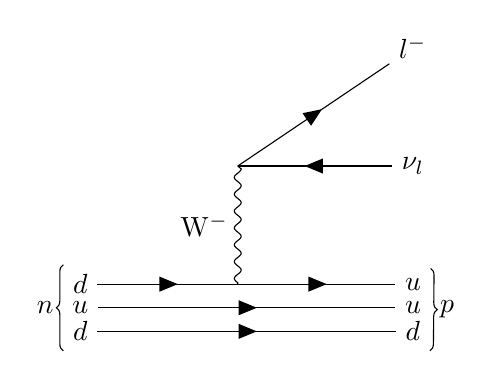
\begin{tikzpicture}
            \begin{feynman}
                \vertex (n1a) {\(d\)};
                \vertex[right=2cm of n1a] (n1b);
                \vertex[right=2cm of n1b] (p1) {\(u\)};

                \vertex[below=0.3cm of n1a] (n2) {\(u\)};
                \vertex[below=0.3cm of n2] (n3) {\(d\)};

                \vertex[below=0.3cm of p1] (p2) {\(u\)};
                \vertex[below=0.3cm of p2]  (p3) {\(d\)};

                \vertex[above=of n1b] (w);

                \vertex[above=of p1] (ln) {\(\nu_l\)}; 
                \vertex[above=of ln] (lc) {\(l^{-}\)}; 

                \diagram* {
                    (n1a) -- [fermion] (n1b) -- [fermion] (p1),
                    (n2) -- [fermion] (p2),
                    (n3) -- [fermion] (p3),
                    (n1b) -- [boson, edge label=\(\W^{-}\)] (w),
                    (w) -- [fermion] (lc),
                    (ln) -- [fermion] (w),
                };
                \draw [decoration={brace}, decorate] (n3.south west) -- (n1a.north west)
                node [pos=0.5, left] {\(n\)};
                \draw [decoration={brace}, decorate] (p1.north east) -- (p3.south east)
                node [pos=0.5, right] {\(p\)};
            \end{feynman}
            \end{tikzpicture}
            \qquad\qquad
            \feynmandiagram [layered layout, horizontal=a to b] {
                a [particle=\(\mu\)] -- [fermion] b,
                b -- [fermion] d [particle=\(\nu_{\mu}\)],
                b -- [boson, edge label=\(\W^{-}\)] c,
                c -- [fermion] e [particle=\(e\)],
                c -- [anti fermion] f [particle=\(\nu_{e}\)],
            };
            \caption{Long-lived decays of the neutron and muon. Diagram created with~\cite{tikz}}
            \label{sm_llp_processes}
        \end{center} \end{figure}

    In SUSY models, LLPs arise for the same basic reasons, and different SUSY models produce LLPs in different ways. The most straightforward SUSY LLP occurs in models with conserved R-parity, a proposed symmetry that prevents proton decay~\cite{primer}\fxnote{Be prepared to show this. Maybe add some diagrams illustrating proton decay w/o R-parity}. In models with R-parity, the SM particles are assigned R-parity +1 and their superpartners are assigned R-parity -1. Conserving the product of R-parity at each vertex has two immediate phenomenological consequences: (1) sparticles can only be produced in pairs and (2) the lightest supersymmetric particle (LSP) is absolutely stable. A neutral LSP could show up in collider searches as missing energy ($\MET$), making $\MET$ a key signature in many conventional SUSY searches~\cite{primer}.

    On the other hand, models with weakly coupled R-parity violating (RPV) terms produce long-lived but not perfectly stable LSPs~\cite{fate}. A similar situation arises in GMSB models\fxnote{should I describe GMSB?} where the gravitino is the LSP. The coupling between the next-to-LSP (NLSP) and gravitino is inversely proportional to the scale of SUSY breaking, which suppresses the NSLP decay rate and can lead to LLPs~\cite{dimopoulos_low_energy}.

    \fxnote{diagram or eqs for R-parity / RPV?}

    LLPs can also arise from particular SUSY mass spectra. Models in the Split SUSY paradigm, for example, propose that the scalar sparticles are significantly more massive than the gauginos. In these models, the gluino becomes long-lived when its decay to a quark and neutralino is mediated by a highly-virtual squark~\cite{kilian_split}. \fxnote{mention that Split throws out naturalness motivation?} On the other hand, some AMSB models\fxnote{explain AMSB?} predict the winos as the lightest gauginos, which leads to nearly-degenerate LSP and NLSP. The NLSP wino then becomes long-lived when its decay is suppressed by the lack of available phase space~\cite{randall_sundrum_out_of_this_world}.

    \fxnote{show a few SUSY spectra?}

\section{The CMS Detector}\fxnote{Add pictures of everything}
    \subsection{Overview}
        \fxnote{define eta, coordinate system in general}
        \fxnote{Mention that ATLAS is similar, says Andrew}  
        The Compact Muon Solenoid (CMS) detector is designed to reconstruct a variety of particles from collisions at the Large Hadron Collider (LHC), a circular proton-proton collider that ran with center-of-mass energy \SI{7}{\tera\electronvolt} in 2010-11, \SI{8}{\tera\electronvolt} in 2012, and \SI{13}{\tera\electronvolt} from 2015 through to the present\fxnote{cite something}. To meet this goal, CMS combines information from several subdetectors nested radially in and around a \SI{4}{\tesla} superconducting solenoid. All together, CMS is \SI{21.6}{\m} long, \SI{14.6}{\m} across, and weighs approximately \SI{12500}{t}~\cite{cms_experiment}. The subdetectors that make up CMS are shown in Fig.~\ref{cms} and described below.

        \noindent \begin{figure}[htbp] \begin{center}
        \includegraphics[width=0.7\textwidth]{images/cms}
        \caption{The CMS detector~\cite{cms_image}}
        \label{cms}
        \end{center} \end{figure}

    \subsection{Tracker}
        \fxnote{mention that analyses below used pre-upgrade tracker}
        In the region closest to the interaction point, CMS uses a fast, high-granularity silicon tracker to reconstruct tracks and pinpoint primary and secondary vertices. The tracker is subdivided into two regions. Inside \SI{20}{cm}, the pixel tracker  uses smaller\fxnote{than what?} silicon pixels to keep the occupancy near \SI{0.1}{\percent} despite the high\fxnote{specify} particle flux. Outside \SI{20}{\cm}, the silicon strip tracker (SST) achieves similar occupancy with larger silicon strips~\cite{cms_tdr}.\fxnote{check occupancy numbers}  

        The pixel tracker, which was upgraded in winter 2016/17, makes up the innermost layer and features approximately \num{124} million silicon pixels, each of which covers an active area of \num{100} by \SI{150}{\micro\meter^2}. The pixels are spread between four barrel layers (BPix) at $\num{2.9}<\mathrm{r}<\SI{16}{cm}$ and 3 endcap disks (FPix) at $\num{29} < \mathrm{z} < \SI{52}{cm}$. The upgraded pixel tracker, shown in Fig.~\ref{pixel_old_new}, should provide 4-hit tracking out to $\eta < \num{2.4}$ and improved b-tagging over the original pixel tracker despite the increased pileup expected in 2017~\cite{cms_pixel_upgrade}.

        \noindent \begin{figure}[htbp] \begin{center}
            \includegraphics[width=0.4\textwidth]{images/pixel_old_new}
            \caption{Diagram showing barrel pixel layers before and after the winter 2016/17 upgrade.~\cite{pixel_old_new}}
            \label{pixel_old_new}
        \end{center} \end{figure}
        
        Just outside the pixel tracker, the silicon strip tracker (SST) occupies the $\num{20} < r < \SI{116}{cm}$ and $\lvert z \rvert < \SI{282}{cm}$ region of CMS. Composed of \num{9.3} million silicon strips that vary in size \fxnote{look up and specify} depending on particle flux in the region, the SST covers an active area of roughly \SI{196}{m^2}. At each trigger, the strip output voltage is read out via optical link~\cite{cms_pixel_upgrade}.

    \subsection{Electromagnetic Calorimeter}
        \fxnote{I define EE \& EB but never use those definitions}
        After traversing the inner tracker, particles next encounter the electromagnetic calorimeter (ECAL). As a homogeneous scintillation calorimeter, ECAL uses \num{61200} lead tungstate crystals in the barrel and \num{7324} in each endcap to reconstruct the energy deposited during electromagnetic showers. Lead tungstate crystals allow for a fast (\SI{80}{\percent} of light within \SI{25}{\nano\s}), compact (radiation length = \SI{0.89}{cm}), fine-grained (Moli\`ere radius = \SI{2.2}{cm}), and radiation hard (up to 10 Mrad\fxnote{learn context for this number}) calorimeter. The main drawback is the relatively low light yield (\SI{30}{photon\per\mega\electronvolt}), which necessitates photodetectors with intrinsic gain that work in magnetic fields\cite{cms_experiment, cms_tdr}.

        The barrel section (EB) extends radially from \num{129} to \SI{177}{cm} and covers a pseudorapidity range of \num{0} to \num{1.479}. The crystals are tapered to approximately project back to the IP\fxnote{define if not already} but not so perfectly that likely particle trajectories align with cracks. Each crystal is approximately one Moli\`ere radius wide and 25.8 radiation lengths deep.

        The crystals in each endcap section (EE) are arranged in an x-y grid that starts at $\lvert z \rvert = \SI{315}{cm}$ and covers a pseudorapidity range of \num{1.479} to \num{3.0}. Additionally, a preshower detector, which consists of two planes of silicon strip detectors and a lead absorber, sits just inside the grid of lead tungstate crystals. \fxnote{Say what the preshower is for? Is it for pi0 rejection? If so, how and why?}

    \subsection{Hadronic Calorimeter}
        \fxnote{define HB \& HF never to be used}
        The hadronic calorimeter (HCAL) uses \SI{3.7}{mm} plates of plastic scintillator interspersed within brass absorber to reconstruct the energy deposited during hadronic showers. Embedded wavelength-shifting fibers capture the scintillation light and transfer it to clear fibers to be read out by hybrid photodiodes\cite{cms_experiment, cms_tdr}.

        The barrel section (HB) spans a pseudorapidity range of \num{-1.4} to \num{1.4} and has \num{2304} towers \fxnote{check}, each of which contains \num{14} \fxnote{check} brass plates and covers an area of \num{0.087} x \SI{0.087}{in} $\eta-\phi$ \fxnote{get a feel for this area}. In addition, an extra layer (or two at $\eta = \num{0}$) of scintillator tiles sits just outside the solenoid. This extra layer, known as hadron outer (HO), spans a pseudorapidity range of \num{-1.26} to \num{1.26} and increases the minimum effective HCAL interaction length to greater than \num{11.8}.

        Each endcap spans a pseudorapidity range of \num{1.3} to \num{3.0} with \num{14} towers in eta and \num{5} to \SI{10}{\degree} $\phi$ segmentation. Also, a steel and quartz fiber forward calorimeter (HF) sits \SI{11.2}{m} from the interaction pipe in a pseudorapidity range of \num{3.0} to \num{5.0}. In HF, particles produce Cherenkov light when traversing the quartz fibers that run parallel to the beamline. \fxnote{say why HF is useful or mention crazy flux?}

    \subsection{Solenoid}
        CMS employs a \SI{4}{T} superconducting solenoid to aid in the measurement of charged particle momenta. The solenoid consists of \num{2168} turns of Nb-Ti superconducting cable and has an inner diameter of \SI{6}{m} and a length of \SI{12.5}{m}. The flux returns through an iron yoke that also houses the muon system. The significant \fxnote{quantify?} bending power helps CMS meet its physics goals of unambiguous sign determination and momentum resolution of \SI{10}{\percent} for muons up to \SI{1}{\tera\electronvolt}\cite{cms_experiment}.

    \subsection{Muon System}
        \fxnote{Specifically mention CMS design specs to meet physics goals?}
        The muon system (MS), which is the outermost subdetector, detects muons with \num{3} varieties of gaseous ionization detectors: drift tubes (DTs) in the barrel, cathode strip chambers (CSCs) in the endcaps, and resistive plate chambers (RPCs) in both the barrel and endcaps. The choice of detector varies between barrel and endcap due to the difference in neutron-induced background\fxnote{what?} , muon rates, and magnetic field strength\fxnote{why does B matter?}. The RPCs are useful in the endcaps and barrel because their fast response and good time resolution allow unambiguous bunch crossing identification. Combining MS and tracker measurements improves the muon momentum resolution at high momenta where the tracker resolution declines \fxnote{quantify or show std plot?}\cite{cms_experiment, cms_tdr}.

        In the barrel detector (BD), four layers of DTs and RPCs are embedded in the solenoid return yoke at \num{4.0}, \num{4.9}, \num{5.9}, and \SI{7.9}{m}. The maximum drift length is \SI{2}{\cm} and the single point resolution is \SI{200}{\cm}. When reconstructing a vector describing the muon momentum, the $\phi$ precision is better than \SI{100}{\micro\m} in position and \SI{1}{\milli\radian} in direction. 

        Each muon endcap detector (ME) is composed of four layers of CSCs and three layers of RPCs. Each CSC has six gas gaps with radial cathode strips and nearly perpendicular planes of anode wires. The wire signal from the ionization-induced electron avalanche is fast enough to use in the L1 trigger, while the slower \fxnote{quantify} cathode strip signal provides precise \fxnote{quantify} position measurements. All in all, the CSC spacial resolution is approximately \SI{200}{\micro\m} and the angular resolution is approximately \SI{10}{\milli\radian}.

    \subsection{Trigger}
        \fxnote{Is entire detector read out at L1?}
        The trigger reduces the data writing rate from the \SI{40}{\mega\hertz} collision rate to less than \SI{1}{\kilo\hertz} so that events can be written to tape. The rate reduction happens in two stages: Level-1 (L1) and High-Level Trigger (HLT). L1 analyzes input from ECAL, HCAL, and MS with custom electronics to reduce the rate to $\approx$100 kHz in 3.8 us. The HLT then uses a dedicated processor farm to further reduce the rate to the desired $<$ 1 kHz\cite{cms_experiment, cms_trigger_upgrade}.

\section{LHC Searches for Long-lived Particles} \label {analyses}
    \fxnote{mention which data was used for each search} 
    \subsection{Overview}
        LLPs leave distinct signatures that differentiate them from SM backgrounds but also add complexity to LLP analyses. CMS and ATLAS were mainly designed to reconstruct stable particles from prompt decays, so LLP searches are often forced\fxnote{the searchers are forced, not the searches} to stray from the traditional analysis path in terms of object reconstruction and background estimation. This report focuses on four complementary LLP signatures: displaced vertices, disappearing tracks, low-velocity particles, and particles that come to a stop before decaying. See Fig.~\ref{jamie_cartoon} for a cartoon of several possible LLP signatures\fxnote{probably a better way to word this sentence}.

        \noindent \begin{figure}[htbp] \begin{center}
        \includegraphics[width=0.7\textwidth]{images/jamie_cartoon}
        \caption{Diagram of several LLP topologies. Image courtesy of Jamie Antonelli}
        \label{jamie_cartoon}
        \end{center} \end{figure}

        Displaced vertex and disappearing track analyses both look for\fxnote{again, analysts look, not analyses} particles that are unstable on detector timescales. Displaced vertex searches are sensitive to LLPs that decay to visible particles within the inner volume \fxnote{specify} of the detector, leaving tracks that point back to a vertex some measurable distance from the nominal interaction point (IP)~\cite{atlas_displaced}. Disappearing track searches are sensitive to LLPs that decay to particles that are either neutral or too soft to be reconstructed~\cite{atlas_disappearing}. Together, these two types of analyses cover a wide range of lifetimes and topologies for LLPs that decay on detector timescales\fxnote{dangerous as hell. Be really good at giving a quantitative explanation of this sentence}\fxnote{find something to cite}.

        Slow and stopped particle searches, on the other hand, are sensitive to detector-stable\fxnote{define?} LLPs that are far more massive\fxnote{be able to quantify} than any stable SM particle. The lower velocity of these high-mass particles can show up as increased ionization energy loss per unit distance ($\langle\frac{dE}{dx}\rangle$) or longer time-of-flight (TOF) measurements than SM particles, which generally have $\beta > \num{0.9}$\fxnote{check this number}~\cite{cms_hscp}. Stopped particle searches take this idea one step further and look for particles that actually come to rest inside the detector before decaying, a phenomenon that could be possible with long lifetimes and small initial kinetic energy\fxnote{how long and how small?}. These analyses look for calorimeter energy deposits or hits in the muon system that are out of time with proton bunch crossings~\cite{cms_stopped}.

        These\fxnote{I've been saying `these' a lot recently} four approaches cover a wide\fxnote{how wide} range of LLP lifetimes that would be missed in traditional searches. The next sections will examine a recent example of each analysis type from either ATLAS or CMS.

    \subsection{Displaced Vertices}
        LLPs that decay before reaching the inner tracker can be identified with a displaced vertex (DV)\fxnote{DVs defined clearly enough in overview?}\fxnote{Is it still a DV if it decays in active material somewhere?}. ATLAS performs a search for such particles by looking for at least one DV along with large MET and large track multiplicity~\cite{atlas_displaced}.\fxnote{make sure I can explain why met and multiplicity} The search is sensitive to LLPs with lifetimes in the \SI{20}{\pico\s} to \SI{10}{\nano\s} range\fxnote{Am I defining sensitivity range consistently across analyses?}.

        This search\fxnote{repetitive wording} uses a simplified benchmark model in the Split SUSY paradigm where gluinos are kinematically accessible but squarks are not. The relevant process, shown in Fig.~\ref{displaced_process}, is pair-produced gluinos that decay to a quark-\fxnote{how to punctuate?}virtual squark pair. The virtual squark then decays to a quark and the LSP, presumed to be a neutralino\fxnote{have I defined neutralino?}\fxnote{why is this a reasonable assumption?}. The large mass of the intermediate squark suppresses the gluino decay, giving the gluino enough time to form an R-hadron\fxnote{first use. Define here if not in LLP section} that propagates some measurable distance before decaying. 

        \fxnote{Add particle labels} 
        \noindent \begin{figure}[htbp] \begin{center}
        \feynmandiagram [layered layout, horizontal=a to b] {
            a -- [plain, gluon] b,
            b -- [anti charged scalar] c,
            b -- [fermion] d,
            c -- [anti fermion] e,
            c -- [plain, boson] f,
        };
        \caption{Long-lived gluino decay through highly virtual squark. Diagram created with~\cite{tikz}}
        \label{displaced_process}
        \end{center} \end{figure}

        Jets and $\MET$ are reconstructed as in conventional analyses, but displaced vertices demand special care when identifying tracks. The standard ATLAS tracking algorithm constrains the transverse and longitudinal impact parameters ($\mathrm{d}_0$ and $\mathrm{z}_0$, respectively) of potential tracks, so the authors employ an additional algorithm, referred to as large-radius tracking (LRT). LRT is run after the standard tracking algorithm and uses only hits that were not used in standard track reconstruction. By relaxing requirements on $\mathrm{d}_0$, $\mathrm{z}_0$, and number of hits, LRT is able to reconstruct tracks that point back to DVs.
        
        Because no SM process produces events that meet the mass and track multiplicity requirements on the DV, only instrumental backgrounds are considered. Specifically, the authors consider hadronic interactions in detector material, incorrectly combined vertices from short-lived SM particles, and hits from unrelated tracks that are incorrectly added to low-mass vertices\fxnote{unnecessary details? I need to get better at explaining this} .

        The authors minimize the effect of hadronic interactions by vetoing the material-dense regions of the detector (see Fig.~\ref{material_map}) and estimate the residual background by extrapolating from the low-mass region, which is dominated by hadronic interactions. After a dedicated study, the background from merged vertices was found to be negligible. Finally, the background from crossing tracks is determined from a model that adds pseudo-tracks to data vertices.

        \noindent \begin{figure}[htbp] \begin{center}
        \includegraphics[width=0.6\textwidth]{images/material_map}
            \caption{Map of material dense regions of the ATLAS detector.\fxnote{explain more}~\cite{atlas_displaced}}
        \label{material_map}
        \end{center} \end{figure}

        After estimating $\num{0.02} \pm \num{0.02}$ background events, exactly zero are observed. The result is then interpreted as an upper limit on the gluino mass and pair-production cross section as a function of gluino lifetime, shown in Fig.~\ref{displaced_limit}. For an LSP neutralino mass of \SI{100}{\giga\electronvolt}, the gluino mass limit is approximately \SI{2000}{\giga\electronvolt} for lifetimes in the \SI{20}{\pico\s} to \SI{10}{\nano\s} range.

        \noindent \begin{figure}[htbp] \begin{center}
        \begin{subfigure}[htbp]{0.45\textwidth} \begin{center}
        \includegraphics[width=\textwidth]{images/displaced_cross_section_limit}
        \end{center} \end{subfigure}
        \begin{subfigure}[htbp]{0.45\textwidth} \begin{center}
        \includegraphics[width=\textwidth]{images/displaced_mass_limit}
        \end{center} \end{subfigure}
            \caption{Limits on the gluino pair-production cross section (left) and gluino mass as a function of lifetime (right)~\cite{atlas_displaced}.}
        \label{displaced_limit}
        \end{center} \end{figure}

    \subsection{Disappearing Tracks}
        Certain models with nearly mass-degenerate LSP and NLSP have the potential to present a remarkable signal: charged particles that seem to disappear in the tracker. Specifically, models with winos as the lightest gauginos\fxnote{have these words been defined?}, such as many AMSB models\fxnote{why amsb? what is amsb?}, will have a chargino NLSP with an observable lifetime (\SI{0.2}{\nano\s} is a typical estimate\fxnote{why? how typical?}) that eventually decays to the neutralino LSP and, commonly, a pion\fxnote{why?}. The nearly-degenerate masses have two important phenomenological roles: (1) increase the chargino lifetime, and (2) ensure low-momentum decay products. The low-momentum pion is then unlikely to be reconstructed, which results in a disappearing track~\cite{atlas_disappearing}.

        Both ATLAS and CMS looked for disappearing tracks during Run I, but the tracker improvements installed in ATLAS before 2015 datataking and CMS before 2017 datataking should increase sensitivity to decays at shorter radii \fxnote{I haven't mentioned previous iterations when talking about other analyses}. The ATLAS search presented here is sensitive to LLP lifetimes of approximately \SI{10}{\pico\s} to \SI{10}{\nano\s} \fxnote{make sure I'm talking about lifetime sensitivity in the same way across analyses}.

        The authors consider two signal processes, both shown in Fig.\ref{disappearing_processes}: (1) electroweak gaugino production resulting in a disappearing track, an ISR jet, and MET and (2) gluino pair production resulting in a disappearing track, four jets, and MET. Process (1) could be the only gaugino production mode at the LHC if the gluino mass is kinematically inaccessible\fxnote{why?}, but process (2), which leads to chargino production in cascade decays, will be dominant if the gluino mass is within reach.

        \fxnote{ugh, this is too hard. just steal diagram from paper or make in jaxodraw. Maybe even use simulated event instead, but make sure I can draw these if asked?}  
        \noindent \begin{figure}[htbp] \begin{center}
        \begin{subfigure}[htbp]{0.2\textwidth} \begin{center}
        \includegraphics[width=\textwidth]{images/disappearing_ew_process}
        \end{center} \end{subfigure}
        \qquad
        \begin{subfigure}[htbp]{0.2\textwidth} \begin{center}
        \includegraphics[width=\textwidth]{images/disappearing_qcd_process}
        \end{center} \end{subfigure}
        \fxnote{Can't get it to work in tikz-feynman. Just take from paper for now.} 
        %\feynmandiagram [layered layout] {
        %    i1 -- [plain] a [blob],
        %    i2 -- [plain] a,
        %    a -- [plain, boson] b [blob],
        %    a -- [plain] f1,
        %    a -- [plain, boson] f2,
        %    b -- [plain, boson] f3,
        %    b -- [scalar] f4,
        %};
            \caption{Benchmark signal processes: electroweak gaugino production (left) and gluino pair-production (right)~\cite{atlas_disappearing}.}
        \label{disappearing_processes}
        \end{center} \end{figure}

        Disappearing track candidates, called pixel tracklets, are selected with a looser track reconstruction algorithm that runs over hits that were not associated to tracks by the standard reconstruction algorithm. The pixel tracklets are required to pass several isolation, transverse momentum ($\pT$), and quality requirements such as number of pixel layer hits. Finally, the disappearing tracks are selected by requiring exactly zero associated hits in the subsequent tracking layer. Event selection requires one pixel tracklet, no electron or muon candidates (to suppress $\ttbar$ and $\W/\Z + \mathrm{jets}$ processes\fxnote{why? be able to explain}), and the $\MET$ and jet requirements associated with either of the two production modes described above\fxnote{be able to explain} .
        
        Pixel tracklets can be faked by random combinations of unrelated hits from nearby particles or by tracks whose pixel hits and next tracking layer hits are not properly associated, either due to a hadron suffering a hard scatter or a lepton radiating a hard photon. These backgrounds come primarily from $\ttbar$ and $\W/\Z + \mathrm{jets}$ processes, and estimates for each type of background are obtained from data. \fxnote{I initially wrote a whole big thing about how each bg was estimated, but I'm thinking it was overkill}

        No excess over expected background is observed, so upper limits are placed in the NLSP chargino mass-lifetime plane for the EW signal process and in the NLSP chargino mass-gluon mass plane for the QCD production process. Fig.~\ref{disappearing_limits} shows the limits for both processes.

        \noindent \begin{figure}[htbp] \begin{center}
        \begin{subfigure}[htbp]{0.3\textwidth} \begin{center}
        \includegraphics[width=\textwidth]{images/disappearing_ew_limit}
        \end{center} \end{subfigure}
        \begin{subfigure}[htbp]{0.3\textwidth} \begin{center}
        \includegraphics[width=\textwidth]{images/disappearing_qcd_200ps_limit}
        \end{center} \end{subfigure}
        \begin{subfigure}[htbp]{0.3\textwidth} \begin{center}
        \includegraphics[width=\textwidth]{images/disappearing_qcd_1ns_limit}
        \end{center} \end{subfigure}
            \caption{Limits on chargino mass and lifetime in the electroweak production channel (left) and gluino and chargino masses in the gluon pair-production channel with a \SI{0.2}{\nano\s} (center) and \SI{1.0}{\nano\s} chargino lifetime.~\cite{atlas_disappearing}}
        \label{disappearing_limits}
        \end{center} \end{figure}

    \subsection{Stopped Particles}
        \fxnote{Add calorimeter search?}  
        \fxnote{too redundant with overview?}
        With long enough lifetimes and sufficient mass, LLPs could come to rest in the detector before decaying. The eventual decay would then lead to energy deposits in the calorimeters or hits in the muon system that could be out of time with proton bunch crossings. A recent CMS analysis looked for such a signal in dimuon final states using the full 2015 and 2016 datasets~\cite{cms_stopped}. 

        This analysis is interpreted in the context of two potential LLPs: gluinos and multiply charged massive particles (mchamps). Long-lived gluinos can appear in models such as Split SUSY, where the squarks and sleptons are quite heavy, but the gluino is relatively light. After being pair produced, gluinos form R-hadrons\fxnote{have these been defined?} and eventually decay to quark-antiquark pairs along with NLSP neutralinos, which then decay to LSP neutralinos along with muon-antimuon pairs. This process is exactly the same as in Fig.~\ref{displaced_process}, but in this case the gluino has enough time to form R-hadrons\fxnote{double check}. The gluino decay is suppressed by the large squark mass, which leads to its appreciable lifetime.

        This analysis uses the muon system to look for pairs of muons that arrive out of time with bunch crossings. The main backgrounds to such a signal are cosmic muons, beam halo\fxnote{explain}, and muon system noise. Beam halo and muon system noise are easily removed by selection criteria, but distinguishing signal from cosmic muons requires a more nuanced approach. After generating signal MC\fxnote{defined?} and modeling cosmic muons from data obtained in dedicated cosmic runs, the authors found that cosmic muons and signal could be differentiated using TOF information from the muon system RPCs and DTs. Essentially, the direction of muon momentum could be gleaned from the timing information, and the authors required outgoing muons in both the upper and lower hemispheres. Fig.~\ref{stopped_muon_differentiation} shows how muons from stopped particles are differentiated from cosmic muons.
        
        \fxnote{check if tof, beta, or bx is better} 
        \noindent \begin{figure}[htbp] \begin{center}
        \includegraphics[width=\textwidth]{images/stopped_reject_cosmic_tof}
            \caption{Cosmic muon rejection using time-of-flight information from the muon system.~\cite{cms_stopped}}
        \label{stopped_muon_differentiation}
        \end{center} \end{figure}

        In addition to the above criteria, the authors developed a new muon reconstruction algorithm, called displaced standalone (DSA), that uses only muon system hits and does not constrain the location of the primary vertex in any way. The full selection requires exactly one good DSA track in each hemisphere with $\pT$ greater than \SI{50}{\giga\electronvolt}, no reconstructed vertices\fxnote{why?}, and several criteria related to the quality of the reconstructed track and timing measurement. Finally, restrictions on the direction of muon momentum (incoming vs outgoing), relative time measurements, and maximum number of CSC hits (0) minimize background from beam halo and cosmic muons\fxnote{be able to explain how}.

        After estimating the background by extrapolating data from the cosmic-enriched\fxnote{enriched how? be able to explain} region to the signal region and determining systematic uncertainties related to the MC simulation, trigger acceptance, and luminosity, the authors calculate the expected background for LLP lifetimes ranging from \SI{100}{\nano\s} to \SI{1}{\micro\s}. In all cases, the expected background is less then one event. Exactly zero events are observed in every lifetime scenario. As shown in Fig.~\ref{stopped_limits}, these results are then interpreted as upper limits on the signal production cross section and mass\fxnote{mass of what?}, which are the first limits for stopped particles that decay to muons at the LHC.

        \fxnote{ok to skip mchamp? Be able to explain why} 
        \noindent \begin{figure}[htbp] \begin{center}
        \begin{subfigure}[htbp]{0.5\textwidth} \begin{center}
        \includegraphics[width=\textwidth]{images/stopped_limit_gluino_cross_section}
        \end{center} \end{subfigure}
        \begin{subfigure}[htbp]{0.45\textwidth} \begin{center}
        \includegraphics[width=\textwidth]{images/stopped_limit_gluino_mass}
        \end{center} \end{subfigure}
            \caption{Upper limits on production cross section as a function of gluino lifetime (left) and mass (right)~\cite{cms_stopped}}
        \label{stopped_limits}
        \end{center} \end{figure}

    \subsection{Heavy Stable Charged Particles}
        Particles that live for more than a couple \SI{}{nano\s}\fxnote{Check this and be more exact} will appear stable in CMS and ATLAS because they can traverse the entire detector before decaying. If such a particle is also sufficiently massive, it can be categorized as a heavy stable charged particle (HSCP). HSCPs are characterized by a greater rate of energy loss via ionization due to the lower speed with which they pass through detector material\fxnote{redundant w/ overview. Probably better explained here than there}. Additionally, HSCPs can be fractionally, singly, or multiply charged, which also affects their rate of energy loss, as shown in Fig.~\ref{hscp_dedx}~\cite{cms_hscp}.

        \noindent \begin{figure}[htbp] \begin{center}
        \includegraphics[width=0.4\textwidth]{images/hscp_dedx}
            \caption{Ionization energy loss as a function of momentum for particles of varying mass and charge~\cite{cms_hscp}}
        \label{hscp_dedx}
        \end{center} \end{figure}

        HSCPs will often be misidentified or missed entirely by standard reconstruction algorithms and analysis criteria, which tend to assume $\beta \approx \num{1}$ and $\lvert q \rvert = e$. Inverting these assumptions provides two handles for a dedicated HSCP search in the context of three benchmark models\fxnote{do I need figures for these?}: (1) HSCPs that form R-hadrons that either change the sign of their electric charge or become neutral before reaching the MS, (2) lepton-like HSCPs (quasi-stable sleptons) that are produced either through decays of squarks or gluinos or directly if squarks and gluinos are kinematically inaccessible, and (3) long-lived lepton-like fermions with arbitrary electric charge. This discussion will focus on the first two models, as they bear more directly on naturalness and SUSY\fxnote{why?}.

        \fxnote{I could talk about how low-beta tracks will show up as zig-zags in DTs b/c reconstruction assumes $\beta \approx \num{1}$. Zig-zag offset is used to estimate beta. Not sure where to fit it in.} \fxnote{Worth mentioning tracker-only vs tracker+TOF?}

        The trigger requires all events to have either a high-$\pT$ muon or large $\MET$. The high-$\pT$ muon trigger is more efficient for all benchmark models except the case where the R-hadron becomes neutral before reaching the MS. In the case where the R-hadron does not leave a track in the MS, the large MET trigger should recover some events.\fxnote{Clunky wording}  

        The authors estimate the signal-region background using an ABCD method in which events are binned in a 2-D plane with uncorrelated axes and the ratio of events in two control regions is used to extrapolate into the signal region from a third control region \fxnote{Do I need to explain this? I glossed over the fact that they used both an ABCD and an ABCDEFGHI}. Systematic uncertainties are introduced in background estimation, signal acceptance, and integrated luminosity.

        No significant excess over predicted background is observed, so the results are interpreted as upper limits in the production cross section - mass plane for the considered models. By comparing the observed limits and theoretical predictions, the authors also extract mass limits for the gluinos, stops, and staus in various models, as shown in Fig.~\ref{hscp_limits}.

        \fxnote{I show separate trk, trk+tof limits but never explain that in text} 
        \noindent \begin{figure}[htbp] \begin{center}
        \begin{subfigure}[htbp]{0.4\textwidth} \begin{center}
        \includegraphics[width=\textwidth]{images/hscp_limit_tracker_only}
        \end{center} \end{subfigure}
        \begin{subfigure}[htbp]{0.4\textwidth} \begin{center}
        \includegraphics[width=\textwidth]{images/hscp_limit_tracker_tof}
        \end{center} \end{subfigure}
        \caption{Production cross section limits on several particles as a function of mass for the tracker-only and tracker+TOF analyses~\cite{cms_hscp}}
        \label{hscp_limits}
        \end{center} \end{figure}

\section{Experimental Viability of Natural SUSY}
    Interpreting current limits in the context of naturalness requires some set of criteria that determine if a model is natural. No well-defined, universally-agreed-upon criteria exist, but certain themes recur in many discussions of natural model building~\cite{craig, vestiges, evans_toward_full, feng, cornering, kim}. The following discussion lays out a simplistic set of criteria for natural SUSY models and attempts to assess the status of natural SUSY in light of current experimental limits\fxnote{Did I just steal Chris's language?}.
    
    \fxnote{I should be able to combine or reorganize the next two paragraphs to flow better} 
    The parameters of interest are the Higgsino\fxnote{careful - do I mean lightest higgsino?}, stop, and gluino masses, which correct the Higgs mass at tree-level, one-loop, and two-loops, respectively (see Eqs.~\ref{higgsino_correction}-\ref{gluino_correction}). Furthermore, the stop and gluino masses are correlated --- a large difference between the two would itself be unnatural~\cite{cornering}.

    \fxnote{define \mu, Q?} 
    \fxnote{make sure these are logically and notationally consistent w/ earlier higgs corrections} 
    \noindent \begin{equation}
        \delta \mHiggs^2 = \mu^2
        \label{higgsino_correction}
    \end{equation}
    \noindent \begin{equation}
        \delta \mHiggs^2 \approx - \frac{3}{8\pi^2} y_t^2 m_{\tilde{t}}^2 \ln{\left(\frac{\Lambda}{Q}\right)}
        \label{stop_correction}
    \end{equation}
    \noindent \begin{equation}
        \delta \mHiggs^2 \approx - \frac{g_3^2 y_t^2}{4\pi^4} M_3^2 \ln{\left(\frac{\Lambda}{Q}\right)}^2
        \label{gluino_correction}
    \end{equation}

    Natural SUSY scenarios, then, are most likely to be constrained by limits on the stop, gluino, and Higgsino masses. The Higgsino, however, does not carry color charge and is far less likely\fxnote{be able to quantify} to be produced at the LHC, leaving stop and gluino mass limits as the most important general constraints on natural SUSY models. As shown in Eqs.~\ref{stop_correction} and~\ref{gluino_correction}, the size of stop and gluino corrections also depends on $\Lambda$, the messenger scale of SUSY breaking.\fxnote{Make sure I understand this. Messenger scale != breaking scale? What are the consequences of a lower messenger scale?}

    Two qualitative decisions must be made when analyzing the state of naturalness: (1) How best to define the degree of fine tuning in a particular model and (2) what degree of fine tuning is acceptable? A common, but not universal, way to quantify fine tuning is
    
    \noindent \begin{equation}
        \Delta_i = \frac{\partial \ln{\mHiggs^2}}{\partial \ln{\alpha_i}} ,
        \label{fine_tuning}
    \end{equation}

    \noindent where $\alpha_i$ is a particular model parameter and $\Delta_i$ is the degree of fine tuning associated with that parameter. The overall degree of fine tuning for the model can then be assigned as $\max{\left(\Delta_i\right)}$~\cite{cornering}.

    Determining the acceptable degree of fine tuning is even more subjective. Before null results and serious constraints started rolling in, it was common to refer to the $\Delta \lesssim 10$ regions of parameter space as natural, but as models are constrained, physicists seem willing to accept greater degrees of fine tuning. Feng proposes an interesting way to recast this problem: instead of asking which regions of parameter space are most natural, physicists should instead ask themselves, ``If superpartners were discovered, what level of fine tuning would be sufficient to convince me that the gauge hierarchy problem is solved by supersymmetry and I should move on to researching other problems?"\fxnote{paraphrase for brevity?} Anecdotally, fine tuning thresholds tend to increase when the question is posed in this way~\cite{feng}.

    Exact upper limits on natural sparticle masses are therefore hard to come by. A somewhat typical set of values is given in~\cite{drees_kim}: $m_{\tilde{H}} \lesssim \SI{500}{\giga\electronvolt}$, $m_{\tilde{t}} \lesssim \SI{1.5}{\tera\electronvolt}$, and $m_{\tilde{g}} \lesssim \SI{3}{\tera\electronvolt}$. Fig.~\ref{atlas_susy_summary} summarizes current SUSY limits from ATLAS searches (CMS limits are generally similar, but a recent plot is not available). Upon inspection, one sees that experimental limits are starting to push on naturalness bounds in many scenarios.

    \fxnote{what do I cite?}  
    \noindent \begin{figure}[htbp] \begin{center}
    \includegraphics[width=0.7\textwidth]{images/atlas_susy_summary}
    \caption{Summary of current experimental limits on SUSY models from ATLAS searches.}
    \label{atlas_susy_summary}
    \end{center} \end{figure}

    Each of the limits in Fig.~\ref{atlas_susy_summary} comes with a particular set of assumptions, making it difficult to draw general conclusions. Some authors try to solve this problem by recasting analyses in terms of a few simplified models that illustrate much of the natural SUSY landscape. Fig.~\ref{cornering_limits} shows the results from one such attempt using $\approx \SI{15}{\femto\barn^{-1}}$ of \SI{13}{\tera\electronvolt} data for the cases of Effective SUSY, RPV SUSY, and a model that combines RPV with Effective SUSY. The authors find that for $\mu = \SI{100}{\giga\electronvolt}$ and $\Lambda = \SI{20}{\tera\electronvolt}$, a small region of $\Delta < 10$ parameter space is currently viable in all cases but, barring discovery, will be excluded within the next few years\fxnote{check}.
    
        \noindent \begin{figure}[htbp] \begin{center}
        \begin{subfigure}[htbp]{0.3\textwidth} \begin{center}
        \includegraphics[width=\textwidth]{images/cornering_effective_100}
        \end{center} \end{subfigure}
        \begin{subfigure}[htbp]{0.3\textwidth} \begin{center}
        \includegraphics[width=\textwidth]{images/cornering_rpv_100}
        \end{center} \end{subfigure}
        \begin{subfigure}[htbp]{0.3\textwidth} \begin{center}
        \includegraphics[width=\textwidth]{images/cornering_rpv_effective_100}
        \end{center} \end{subfigure}
            \caption{Comparing experimental limits to $\Delta < 10$ naturalness bounds for Effective (left), RPV (center), and Effective+RPV (right) SUSY models ~\cite{cornering}.}
        \label{cornering_limits}
        \end{center} \end{figure}

    As viable parameter space for natural SUSY continues to shrink, it is important to identify and fill in the gaps left by conventional analyses. LLP searches such as those in Sec.~\ref{analyses} do just that by opening up sensitivity to lifetimes that would otherwise be missed. Fig.~\ref{fate_limits}, for example, shows stop mass limits from several Run I LLP searches that have been recast using a simple RPV model~\cite{fate}. By combining results from several analyses, the authors constrain the stop mass for a broad and continuous range of lifetimes that would have been invisible to conventional searches. 

        \noindent \begin{figure}[htbp] \begin{center}
        \includegraphics[width=0.4\textwidth]{images/fate_limits}
        \caption{Limits.~\cite{fate}}
        \label{fate_limits}
        \end{center} \end{figure}

    Many LLP searches are motivated by and interpreted within specific models that predict unique signatures. Approaching analyses is this way often results in nearly background-free searches with good signal acceptance for the model in question, but it can be difficult to draw general conclusions or assess the complementarity (or redundancy) of different searches~\cite{fate}. As the number of LLP searches grows, it will be important to design searches around simplified models that enable researchers to combine and compare results to draw general conclusions.~\cite{evans_talk}.

    Combining results from several searches can also elucidate new directions for important searches. By recasting several LLP searches similar to those described in Sec.~\ref{analyses}, Evans and Shelter looked at the current viability of several SUSY spectra that predict long-lived staus. They identified significant gaps in coverage for models with displaced taus or same-sign displaced leptons, signals that appear in several well-motivated models such as GMSB, where staus are commonly the NLSP, and RPV, where certain couplings lead to same-flavor leptons~\cite{ll_staus}. 

    The uniqueness of LLP signatures and idiosyncrasy of LLP analyses leads to a broad and diverse set of analyses that will surely grow as viable natural parameter space shrinks and more imaginations are turned to filling in the gaps. Fully covering natural SUSY parameter space will take a dedicated effort from the LLP community, both to maximize the reach of individual searches and to design complementary analyses that can be used to draw general conclusions. Although natural SUSY is under pressure from conventional and long-lived null results, it remains one of the least-tuned options for natural BSM physics\fxnote{double check, then cite cornering, feng, nate, and/or giudice}. The next several years will be decisive~\cite{cornering}, and physicists will have to be clever to probe every corner of natural parameter space.

\clearpage
\pagebreak
\singlespacing
\bibliography{draft}{}
\bibliographystyle{unsrt}

\end{document}
